\title{Star Formation and Feedback in Stellar Clusters and Galaxies.\\
       Code performance and scaling.}

\documentclass[11pt]{article}

\usepackage[letterpaper, margin=1in]{geometry}
\usepackage{amsmath}
\usepackage{natbib}
\usepackage{graphicx}
\usepackage{epstopdf}
\epstopdfsetup{update}
\citestyle{aa}

\newcommand {\apj}{ApJ}
\newcommand {\aj}{AJ}
\newcommand {\apjs}{ApJS}
\newcommand {\apjl}{ApJL}
\newcommand {\mnras}{MNRAS}
\newcommand {\aap}{A\&A}
\newcommand {\aapr}{A\&ARv}
\newcommand {\araa}{ARA\&A}
\newcommand {\pasj}{PASJ}
\newcommand {\pasp}{PASP}
\newcommand {\bain}{Bulletin of the Astronomical Institutes of the Netherlands}
\newcommand {\fcp}{Fundamentals of Cosmic Physics}
\newcommand {\nat}{Nature}
\newcommand {\na}{New Astronomy}
\newcommand{\eg}{e.g.,}
\newcommand\rmxaa{Rev. Mex. Astron. Astrofis.} % Revista Mexicana de Astronomia y Astrofisica

\begin{document}
\maketitle

\section{Introduction}



\section{\texttt{Enzo}}

We determine the performance and scaling properties of \texttt{Enzo} in the context of the typical computational loads of our intended isolated dwarf galaxy simulations. In this context, we are only concerned with how \texttt{Enzo} scales in parallel with adaptive mesh refinement (AMR), ignoring its scaling properties for uniform, static grids, and presenting only weak scaling tests at our fiducial resolution. The more general properties of \texttt{Enzo} can be found in the recent method paper \citep{Enzo2014}. We use three case studies to determine the performance and scaling properties of \texttt{Enzo}, two of which are isolated dwarf galaxy simulations conducted at and just below our intended resolution, and the third is a lower resolution run intended to characterize how including radiative transfer affects performance.

\subsection{Performance and Scaling of AMR Simulations}

Understanding the exact scaling and performance properties of an AMR simulation is challenging, as the total number of computational grids can vary significantly over the course of the simulation run. In the case of our dwarf galaxy simulations, the number of grids will initially be relatively insignificant, but will grow substantially as the gas collapses into dense regions and forms stars. Based on our test simulations, we expect the number of grid cells to be roughly consistent from this point onward, fluctuating around some mean value. Given a roughly constant cell count, code performance (number of cell updates per second per processor) will be roughly consistent, with computational expense (SU per simulation Myr) set by the size of each time step. Time steps are determined independently on each refinement level by the Courant-Freidrichs-Lewy, or CFL, condition. For a fixed physical state, the time step scales linearly with cell size, but is inversely proportional to the sum of the sound speed and bulk velocity in a given cell. Therefore, the time step is sensitive to the presence of the hot, fast moving gas created through stellar wind and supernova feedback. Radiative transfer incurs an extra expense in these simulations that correlates with the number of ionizing sources, but depends on both the nature and clustering of the sources (unclustered sources can be more evenly distributed amongst multiple processors). Our explicit implementation of cosmic ray diffusion means that the minimum diffusion time step depends on $\delta x^2$, which can reduce the simulation time step by a factor of 5. We refer to the main document for further details on how this affects the anticipated cost of our simulations.

%\subsection{Code Performance and Grid Hierarchy}

We begin by illustrating how our computational domain is divided between individual levels in an AMR run of our dwarf galaxy. Figure~\ref{fig:levels} shows the results of two test simulations of our dwarf galaxy in the planned production scale box ($16.384^3$ kpc with a $128^3$ root grid) at a maximum refinement level of 6 and 7, corresponding to a physical resolution of 2.0 and 1.0 pc respectively. As demonstrated, the amount of wall time spent on a single cycle is dominated by computation on the highest level of refinement (top left panel). This is because the number of cells on a given level generally increases towards higher levels of refinement (top right panel), with the most cells on a given level at the highest refinement level, and because the time step is allowed to vary on each level, scaling linearly with the cell size. In reality, the typical timestep scales much more steeply with refinement level as the feedback physics (with hot gas and high velocities) is injected at the maximum resolution, and we expect most of the cells in the root grid to be sufficiently far from the galaxy to be devoid of any hot, fast moving gas. 

\begin{figure}
\centering
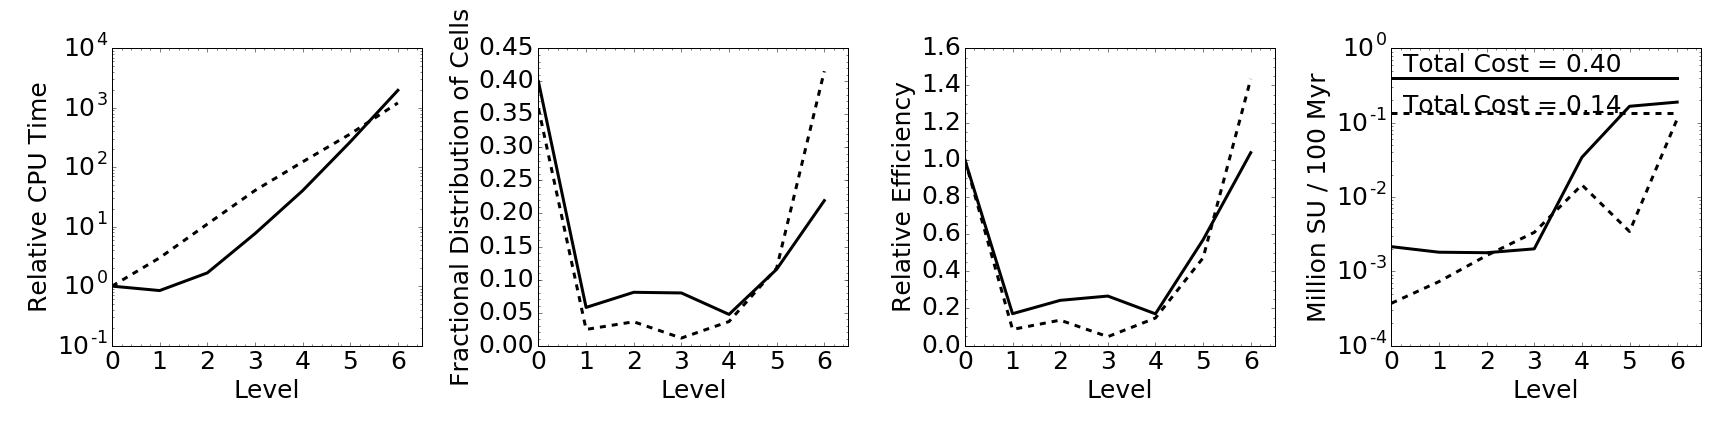
\includegraphics[width=0.95\linewidth]{enzo_levels}
\caption{Break down of grid hierarchy and performance on each level for a two test simulations of our fiducial model at two maximum refinement levels, level 6 (dashed) and level 7 (solid), corresponding to physical resolutions of 2.0 and 1.0 pc respectively. Each was run on the TACC Stampede cluster with 128 processors. Shown is the wall time spent on each level, normalized by the root grid time (top left), the fraction of all cells on each level (top right), the effeciency of each level relative to the root grid, defined as the number of cell updates per second per processor (bottom left), and an estimate for the the theoretical minimum SU cost per Gyr of simulation time. See text for further discussion of each of these points.}
\label{fig:levels}
\end{figure}

The lower left panel of Figure\ref{fig:levels} provides the relative efficiency of each level, as normalized to the efficiency of level 0. We define efficiency as the number of cell updates per second per processor, with typical values of 10$^4$ as averaged over all levels. The efficiency is determined primarily by the ability of \texttt{Enzo} to properly load balance across all processors, which becomes inefficient if there are too few cells on a given level. For example, levels 1 and 2 have low cell counts and low efficiencies; however, low efficiencies for this reason are generally irrelevant, as very little time is actually spent updating these cells. The efficiency at he highest levels of refinement is generally around $2\times 10^4$ cells/s/proc. Assuming all levels can operate completely independently (which is physically impossible), we present the theoretical lower limit cost of 1 Gyr of simulation time per level on 128 cores in the lower right panel; the horizontal line gives the sum over all levels. To compute this, we adopt typical time steps for each level as obtained from our test simulations using only supernovae feedback and stellar winds. This means a typical time step of roughly 300 years at level 7, and 600 years at level 6. In practice, the levels cannot operate independently; a more realistic estimate is a factor of 2-3 larger than this theoretical minimum.

\begin{figure}
\centering
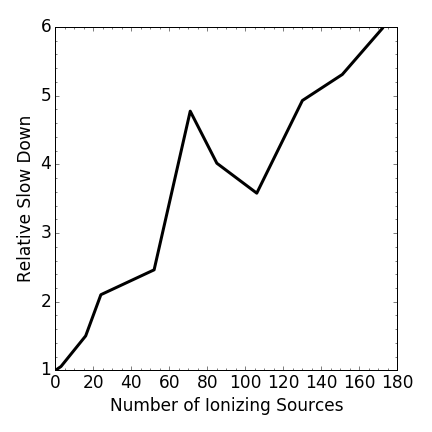
\includegraphics[width=0.45\linewidth]{enzo_radiation}
\caption{Estimate of relative slow down of a test simulation as a function of the number of ionizing sources. The test simulation is of our dwarf galaxy at 8.0 pc resolution, or a maximum refinement level of 4, run on 32 processors on the TACC Stampede cluster. This test simulation included supernovae, stellar winds, photoelectric heating, and radiative transfer. We estimate that there will be at most a few hundred sources at any one moment in our simulation, implying a maximal slow down of about a factor of 10.}
\label{fig:radiation}
\end{figure}

We demonstrate the effects of including radiative transfer as a function of the number of ionizing particles in Figure~\ref{fig:radiation} for a test simulation run with a maximum refinement level of 4 (8.0 pc resolution) on 64 processors. Shown is the slow down of a given cycle as a function of the number of ionizing sources. We compute this as the number of cell updates per second per particle, normalized to the zero particle case. This implicitly assumes that any decrease in performance is due solely to the number of sources, and no other factors. To be clear, the additional computational time incurred by including radiation is split in into three parts, 1) evolving the photon packages through the grid cells, 2) ray tracing from each source to deposit the photon packages, and 3) communication time communicating photon packages between processors. For this reason, the additional cost also depends upon the nature of the sources themselves, their clustering, and the details of the medium the photons propagate through.

\subsection{Scaling Tests}

\begin{figure}
\centering
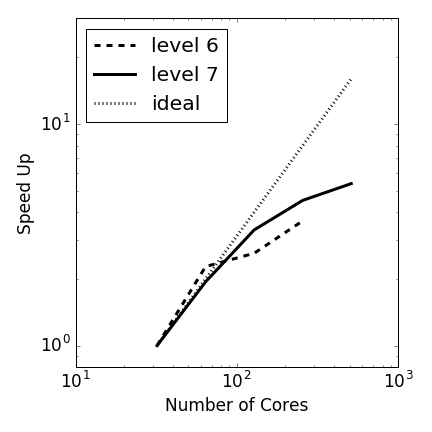
\includegraphics[width=0.45\linewidth]{enzo_scaling}
\caption{A demonstration of weak scaling for our two test runs with maximum refinement levels of 6 (dashed) and 7 (solid). Scaling works very well for up to 128 cores, but becomes less than ideal about this amount. We anticipate to run with either 128 or 256 cores for all of our simulations depending on how the grid and particle count evolve in the simulation.}
\label{fig:scaling}
\end{figure}

We demonstrate weak scaling in Figure~\ref{fig:scaling} for our two test simulations, each run with a maximum of 6 and 7 levels of refinement, as compared to ideal scaling. Our simulations scale well up to about 128 processors, falling away from ideal at higher processor counts. However, this is in part because scaling in \texttt{Enzo} works best when the number of root grids on a side is greater than or equal to the number of cores. In this case, we don't expect perfect scaling much above 128 cores for our 128$^3$ simulations. For this reason, we anticipate to run all of our dwarf galaxy models on 128 or 256 cores depending on how the number of cells and particles varies throughout the simulation. We note that \texttt{Enzo} has been shown to scale well to at least 10$^3$ processors in a variety of contexts.

\bibliographystyle{apj}
\bibliography{msbib}


\end{document}
